\documentclass[tikz]{standalone}

% tikz
\usepackage{tikz, pgfplots}
% i wish external worked but idk it sucks
%\usetikzlibrary{external}
%\tikzexternalize[prefix=figures/]

% for function graph
\usetikzlibrary{positioning}
\usetikzlibrary{shapes.geometric}
\usetikzlibrary{positioning}
\usetikzlibrary{shapes.misc}
\tikzset{
dot/.style = {circle, fill=#1, minimum size=5pt,
              inner sep=0pt, outer sep=0pt},
dot/.default = black % size of the circle diameter
}
\tikzset{cross/.style={cross out, draw=black, minimum size=2*(#1-\pgflinewidth), inner sep=0pt, outer sep=0pt},
%default radius will be 1pt. 
cross/.default={1pt}}

 % for braces
\usetikzlibrary{decorations.pathreplacing}
% for hashing area
\usetikzlibrary{patterns}
% tableaux var, signe
% source https://www.sqlpac.com/fr/documents/latex-package-tkz-tab-tikz-tableaux-de-signes-et-de-variations-de-fonctions.html
\usepackage{tkz-tab}
%%%%%%%%%%%%%%%%%%%%%%%%%%%%%%
% SELF MADE COLORS
%%%%%%%%%%%%%%%%%%%%%%%%%%%%%%


\definecolor{myg}{RGB}{56, 140, 70}
\definecolor{myb}{RGB}{45, 111, 177}
\definecolor{myr}{RGB}{199, 68, 64}
\definecolor{mytheorembg}{HTML}{F2F2F9}
\definecolor{mytheoremfr}{HTML}{00007B}
\definecolor{mylenmabg}{HTML}{FFFAF8}
\definecolor{mylenmafr}{HTML}{983b0f}
\definecolor{mypropbg}{HTML}{f2fbfc}
\definecolor{mypropfr}{HTML}{191971}
\definecolor{myexamplebg}{HTML}{F2FBF8}
\definecolor{myexamplefr}{HTML}{88D6D1}
\definecolor{myexampleti}{HTML}{2A7F7F}
\definecolor{mydefinitbg}{HTML}{E5E5FF}
\definecolor{mydefinitfr}{HTML}{3F3FA3}
\definecolor{notesgreen}{RGB}{0,162,0}
\definecolor{myp}{RGB}{197, 92, 212}
\definecolor{mygr}{HTML}{2C3338}
\definecolor{myred}{RGB}{127,0,0}
\definecolor{myyellow}{RGB}{169,121,69}
\definecolor{myexercisebg}{HTML}{F2FBF8}
\definecolor{myexercisefg}{HTML}{88D6D1}
\definecolor{doc}{RGB}{0,60,110}

% manim colors because they're beautiful
% https://docs.manim.community/en/stable/reference/manim.utils.color.manim_colors.html

\definecolor{BLACK}{HTML}{000000}\definecolor{BLUE}{HTML}{58C4DD}\definecolor{BLUE_A}{HTML}{C7E9F1}\definecolor{BLUE_B}{HTML}{9CDCEB}\definecolor{BLUE_C}{HTML}{58C4DD}\definecolor{BLUE_D}{HTML}{29ABCA}\definecolor{BLUE_E}{HTML}{236B8E}\definecolor{DARKER_GRAY}{HTML}{222222}\definecolor{DARKER_GREY}{HTML}{222222}\definecolor{DARK_BLUE}{HTML}{236B8E}\definecolor{DARK_BROWN}{HTML}{8B4513}\definecolor{DARK_GRAY}{HTML}{444444}\definecolor{DARK_GREY}{HTML}{444444}\definecolor{GOLD}{HTML}{F0AC5F}\definecolor{GOLD_A}{HTML}{F7C797}\definecolor{GOLD_B}{HTML}{F9B775}\definecolor{GOLD_C}{HTML}{F0AC5F}\definecolor{GOLD_D}{HTML}{E1A158}\definecolor{GOLD_E}{HTML}{C78D46}\definecolor{GRAY}{HTML}{888888}\definecolor{GRAY_A}{HTML}{DDDDDD}\definecolor{GRAY_B}{HTML}{BBBBBB}\definecolor{GRAY_BROWN}{HTML}{736357}\definecolor{GRAY_C}{HTML}{888888}\definecolor{GRAY_D}{HTML}{444444}\definecolor{GRAY_E}{HTML}{222222}\definecolor{GREEN}{HTML}{83C167}\definecolor{GREEN_A}{HTML}{C9E2AE}\definecolor{GREEN_B}{HTML}{A6CF8C}\definecolor{GREEN_C}{HTML}{83C167}\definecolor{GREEN_D}{HTML}{77B05D}\definecolor{GREEN_E}{HTML}{699C52}\definecolor{GREY}{HTML}{888888}\definecolor{GREY_A}{HTML}{DDDDDD}\definecolor{GREY_B}{HTML}{BBBBBB}\definecolor{GREY_BROWN}{HTML}{736357}\definecolor{GREY_C}{HTML}{888888}\definecolor{GREY_D}{HTML}{444444}\definecolor{GREY_E}{HTML}{222222}\definecolor{LIGHTER_GRAY}{HTML}{DDDDDD}\definecolor{LIGHTER_GREY}{HTML}{DDDDDD}\definecolor{LIGHT_BROWN}{HTML}{CD853F}\definecolor{LIGHT_GRAY}{HTML}{BBBBBB}\definecolor{LIGHT_GREY}{HTML}{BBBBBB}\definecolor{LIGHT_PINK}{HTML}{DC75CD}\definecolor{LOGO_BLACK}{HTML}{343434}\definecolor{LOGO_BLUE}{HTML}{525893}\definecolor{LOGO_GREEN}{HTML}{87C2A5}\definecolor{LOGO_RED}{HTML}{E07A5F}\definecolor{LOGO_WHITE}{HTML}{ECE7E2}\definecolor{MAROON}{HTML}{C55F73}\definecolor{MAROON_A}{HTML}{ECABC1}\definecolor{MAROON_B}{HTML}{EC92AB}\definecolor{MAROON_C}{HTML}{C55F73}\definecolor{MAROON_D}{HTML}{A24D61}\definecolor{MAROON_E}{HTML}{94424F}\definecolor{ORANGE}{HTML}{FF862F}\definecolor{PINK}{HTML}{D147BD}\definecolor{PURE_BLUE}{HTML}{0000FF}\definecolor{PURE_GREEN}{HTML}{00FF00}\definecolor{PURE_RED}{HTML}{FF0000}\definecolor{PURPLE}{HTML}{9A72AC}\definecolor{PURPLE_A}{HTML}{CAA3E8}\definecolor{PURPLE_B}{HTML}{B189C6}\definecolor{PURPLE_C}{HTML}{9A72AC}\definecolor{PURPLE_D}{HTML}{715582}\definecolor{PURPLE_E}{HTML}{644172}\definecolor{RED}{HTML}{FC6255}\definecolor{RED_A}{HTML}{F7A1A3}\definecolor{RED_B}{HTML}{FF8080}\definecolor{RED_C}{HTML}{FC6255}\definecolor{RED_D}{HTML}{E65A4C}\definecolor{RED_E}{HTML}{CF5044}\definecolor{TEAL}{HTML}{5CD0B3}\definecolor{TEAL_A}{HTML}{ACEAD7}\definecolor{TEAL_B}{HTML}{76DDC0}\definecolor{TEAL_C}{HTML}{5CD0B3}\definecolor{TEAL_D}{HTML}{55C1A7}\definecolor{TEAL_E}{HTML}{49A88F}\definecolor{WHITE}{HTML}{FFFFFF}\definecolor{YELLOW}{HTML}{FFFF00}\definecolor{YELLOW_A}{HTML}{FFF1B6}\definecolor{YELLOW_B}{HTML}{FFEA94}\definecolor{YELLOW_C}{HTML}{FFFF00}\definecolor{YELLOW_D}{HTML}{F4D345}\definecolor{YELLOW_E}{HTML}{E8C11C}

% Schwartz
\renewcommand{\S}{\mathcal{S}} % \S est le signe paragraphe normalement

% corps
\newcommand{\C}{\mathcal{C}}
\newcommand{\R}{\mathbb{R}}
\newcommand{\Rnn}{\mathbb{R}^{2n}}
\newcommand{\Z}{\mathbb{Z}}
\newcommand{\N}{\mathbb{N}}
\newcommand{\Q}{\mathbb{Q}}

% domain
\newcommand{\D}{\mathcal{D}}

% order notations
\renewcommand{\O}{\mathcal{O}}

% japanese bracket
\newcommand{\japb}[1]{\langle #1 \rangle}

% arrows over partial derivatives
\newcommand{\lp}{\overleftarrow{\partial}}
\newcommand{\rp}{\overrightarrow{\partial}}

% quantization
\newcommand{\h}{\hbar}
\newcommand{\Opht}{\textrm{Op}_{\h}^{t}}
\newcommand{\Op}[2][\hbar]{\textrm{Op}_{#1}^{#2}}

% omega functions
\newcommand{\omegap}[2][\rho_0]{\omega(\partial_{#1},\partial_{#2})}
\newcommand{\omegar}[2][\rho_0]{\omega(#1,#2)}
% PLUS INFTY AND MINUS INFTY WITH NO SPACE
\newcommand{\pinfty}{{+}\infty}
\newcommand{\minfty}{{-}\infty}


\tikzset{
	every node/.style = {font=\Large}
}

\begin{document}
%
	% page 1
  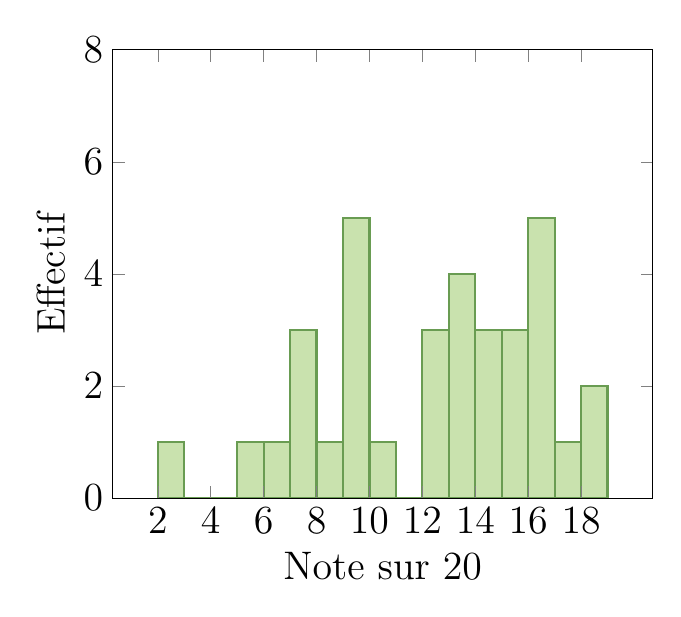
\begin{tikzpicture}[scale=1]
    \begin{axis}[
        ymin=0, ymax=8,
        %minor y tick num = 3,
        xtick = {2, 4, ..., 16, 18},
        area style,
        xlabel = {Note sur $20$},
        ylabel = {Effectif}
      ]
      \addplot+[ybar interval,mark=no, draw=GREEN_E, thick, fill=GREEN_A] plot coordinates {
        (2,1) (3,0) (4,0) (5,1) (6,1) (7,3) (8,1) (9,5) (10,1) (11,0) (12,3) (13,4) (14,3) (15,3) (16,5) (17,1) (18,2) (19,0)
      };
    \end{axis} 
  \end{tikzpicture}
  % page 2
  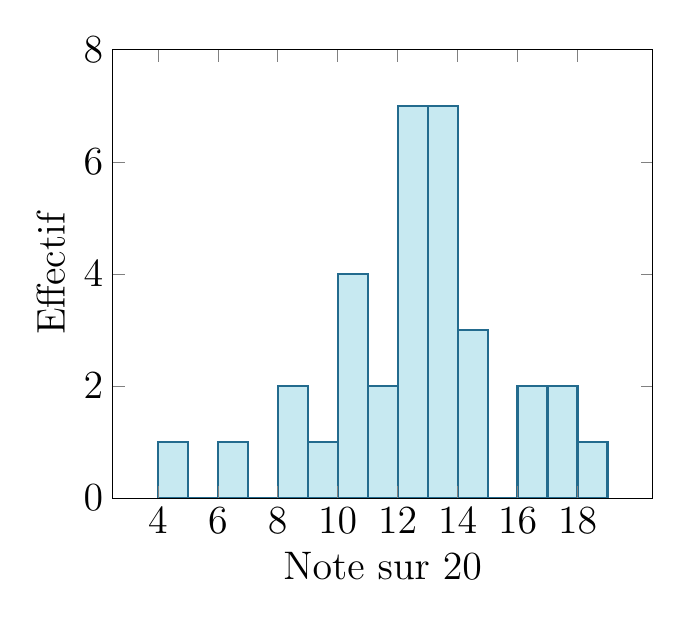
\begin{tikzpicture}[scale=1]
    \begin{axis}[
        ymin=0, ymax=8,
        %minor y tick num = 3,
        %xtick = {4, 5, ..., 18, 19},
        xtick = {2, 4, ..., 16, 18},
        area style,
        xlabel = {Note sur $20$},
        ylabel = {Effectif}
      ]
      \addplot+[ybar interval,mark=no, draw=BLUE_E, thick, fill=BLUE_A] plot coordinates {
        (4,1) (5,0) (6,1) (7,0) (8,2) (9,1) (10,4) (11,2) (12,7) (13,7) (14,3) (15,0) (16,2) (17,2) (18,1) (19,0)
      };
    \end{axis} 
  \end{tikzpicture}
  % page 3
  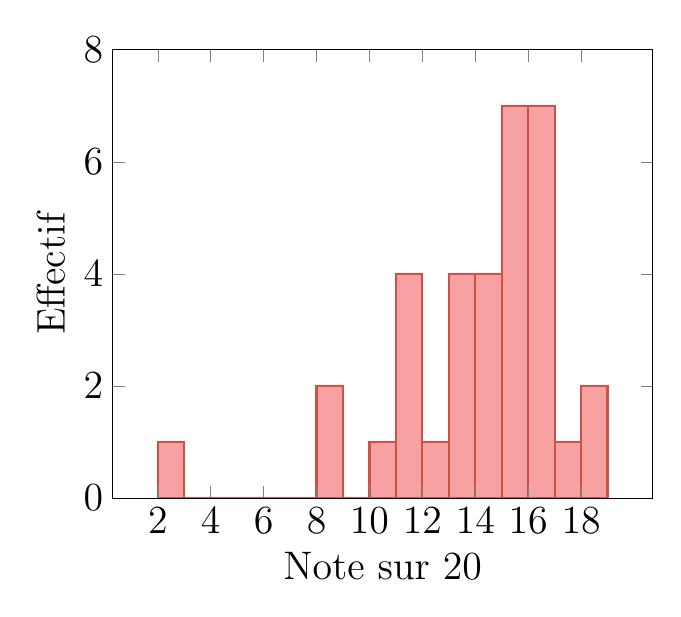
\begin{tikzpicture}[scale=1]
    \begin{axis}[
        ymin=0, ymax=8,
        %minor y tick num = 3,
        xtick = {2, 4, ..., 16, 18},
        area style,
        xlabel = {Note sur $20$},
        ylabel = {Effectif}
      ]
      \addplot+[ybar interval,mark=no, draw=RED_E, thick, fill=RED_A] plot coordinates {
      		(2,1) (3,0) (8,2) (9,0) (10, 1) (11,4) (12,1) (13,4) (14,4) (15,7) (16,7) (17,1) (18,2) (19,0)
      };
    \end{axis} 
  \end{tikzpicture}
  % page 4
  % j'aime pas les pie chart c'est inutile
\def\angle{0}
\def\radius{3}
\def\cyclelist{{"myg","gray","myr","myb"}}
\newcount\cyclecount \cyclecount=-1
\newcount\ind \ind=-1
  \begin{tikzpicture}
      \foreach \percent/\name in {
        75/{préoccupation mineure (LC)},
        6/{données insufficantes (DD)},
        14/{éteintes ou menacées (EX à VU)},
        5/{quasi menacées (NT)}
    } {
      \ifx\percent\empty\else               % If \percent is empty, do nothing
        \global\advance\cyclecount by 1     % Advance cyclecount
        \global\advance\ind by 1            % Advance list index
        \ifnum3<\cyclecount                 % If cyclecount is larger than list
          \global\cyclecount=0              %   reset cyclecount and
          \global\ind=0                     %   reset list index
        \fi
        \pgfmathparse{\cyclelist[\the\ind]} % Get color from cycle list
        \edef\color{\pgfmathresult}         %   and store as \color
        % Draw angle and set labels
        \draw[fill={\color!50},draw={\color}] (0,0) -- (\angle:\radius)
          arc (\angle:\angle+\percent*3.6:\radius) -- cycle;
        \node at (\angle+0.5*\percent*3.6:0.7*\radius) {\percent\,\%};
        \node[pin=\angle+0.5*\percent*3.6:\name]
          at (\angle+0.5*\percent*3.6:\radius) {};
        \pgfmathparse{\angle+\percent*3.6}  % Advance angle
        \xdef\angle{\pgfmathresult}         %   and store in \angle
      \fi
    };
  \end{tikzpicture}
\end{document}